%*=== WARNING! PGF 3.0 of higher required to compile! ===*%
\documentclass[a4paper,11pt]{article}
\usepackage[utf8]{inputenc}
\usepackage{type1cm}
\usepackage[english]{babel}
\usepackage[%hypertex,
                 unicode=true,
                 plainpages = false, 
                 pdfpagelabels, 
                 bookmarks=true,
                 bookmarksnumbered=true,
                 bookmarksopen=true,
                 breaklinks=true,
                 backref=false,
                 colorlinks=true,
                 linkcolor = blue,		% Use "blue" if you want to highlight them
                 urlcolor  = blue,
                 citecolor = red,
                 anchorcolor = green,
                 hyperindex = true,
                 linktocpage = true,
                 hyperfigures
]{hyperref}
\hypersetup{
 pdftitle={Problem set 1, Many-Body Theory},
 pdfauthor={Matteo Seclì <secli.matteo@gmail.com>},
 pdfsubject={Solution to the homework problems for the course "Problems in Electronic Structure"@SISSA, Fall 2016.}
}
\usepackage{amsthm}
\renewenvironment{proof}
	{\noindent\textsc{Solution:}}
	{\begin{flushright}$\blacksquare$\end{flushright}\vskip 1em}
\usepackage{amsmath}
\usepackage{amsfonts}
\usepackage{amssymb}
\usepackage{mathtools}
\usepackage{bbold}
\usepackage{siunitx}
\usepackage{cancel}
\usepackage{braket}
\usepackage{graphicx}
\graphicspath{{figures/PNG/}{figures/PDF/}{figures/}}
\usepackage[all]{xy}
\usepackage{float}
%\usepackage[bottom]{footmisc}
\usepackage{enumitem}
%\usepackage{comment} % Uncomment for selective compilation
\usepackage{geometry}
\usepackage{circuitikz}
\usetikzlibrary{quotes,angles}
\usetikzlibrary{arrows}
\usetikzlibrary{calc,decorations.markings}
\definecolor{myred}{rgb}{0.7,0.1,0.1}
\definecolor{myblue}{rgb}{0,0.447,0.741}
\usepackage{pgfplots}
\pgfplotsset{compat=1.12}
\usepackage{subcaption}
\newcounter{problemsetnumber}
\setcounter{problemsetnumber}{1}
\newtheorem{problem}{Problem}[problemsetnumber]
\newtheorem*{example}{Example}
\newtheorem{theorem}{Theorem}
\let\oldhat\hat
\renewcommand{\vec}[1]{\mathbf{#1}}
%\renewcommand{\hat}[1]{\widehat{\mathbf{#1}}}
%\newcommand{\si}[1]{\mathrm{#1}}
\DeclareMathOperator*{\arsinh}{arsinh}
\makeatletter
\DeclareRobustCommand{\abs}{\@ifstar\@firstofone\@abs}
\newcommand{\@abs}[1]{\left\lvert #1 \right\rvert}
\newcommand{\repeq}{\overset{\mathrm{rep}}{=}}
\makeatother
%\usepackage[square]{natbib}
\newcommand{\Mathematica}{Mathematica\textsuperscript{\textregistered}}
\newcommand{\MATLAB}{MATLAB\textsuperscript{\textregistered}}

\title{SISSA - Solid State Problems\\\smallskip \Large Problem set 1 (week 42)}
\author{Seclì, Shaidu}
\begin{document}

\maketitle

\begin{problem}[A. Graphene model]
	\label{pro:A}
	Refer to the assignment paper for the text of the problem.
\end{problem}
\begin{proof}
	\begin{figure}[H]
		\centering
		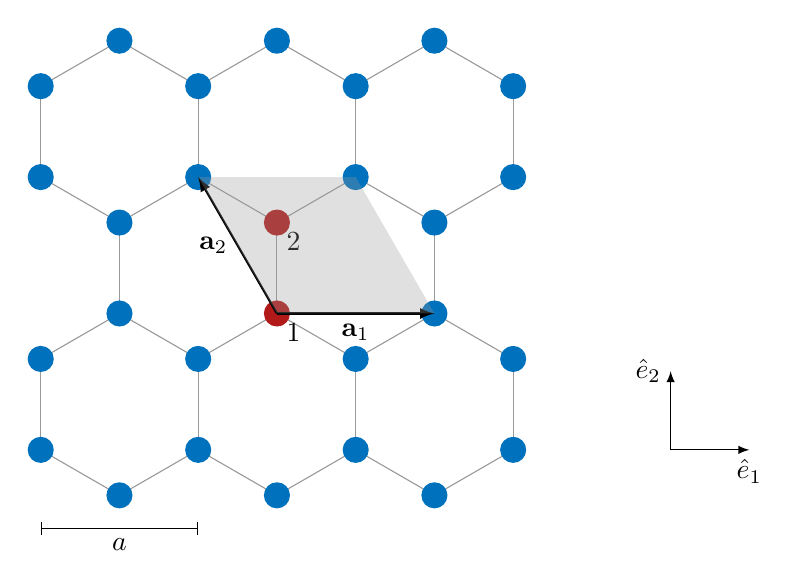
\begin{tikzpicture}[>=latex, scale=1.0, transform shape]
			% Draw the horizontal zig-zag lines and some dots. a=2
			\draw[color=black!40!white] (0,0) -- (1,-{sqrt(3)/3}) node[circle,fill,color=myblue] {} -- (2,0) -- (3,-{sqrt(3)/3}) node[circle,fill,color=myblue] {} -- (4,0) -- (5,-{sqrt(3)/3}) node[circle,fill,color=myblue] {} -- (6,0);
			\draw[color=black!40!white] (0,{2*sqrt(3)/3}) -- (1,{sqrt(3)}) -- (2,{2*sqrt(3)/3}) -- (3,{sqrt(3)}) -- (4,{2*sqrt(3)/3}) -- (5,{sqrt(3)}) -- (6,{2*sqrt(3)/3});
			\draw[color=black!40!white] (0,{2*sqrt(3)}) -- (1,{5*sqrt(3)/3}) -- (2,{2*sqrt(3)}) -- (3,{5*sqrt(3)/3}) -- (4,{2*sqrt(3)}) -- (5,{5*sqrt(3)/3}) -- (6,{2*sqrt(3)});
			\draw[color=black!40!white] (0,{8*sqrt(3)/3}) -- (1,{3*sqrt(3)}) node[circle,fill,color=myblue] {} -- (2,{8*sqrt(3)/3}) -- (3,{3*sqrt(3)}) node[circle,fill,color=myblue] {} -- (4,{8*sqrt(3)/3}) -- (5,{3*sqrt(3)}) node[circle,fill,color=myblue] {} -- (6,{8*sqrt(3)/3});
			
			% Draw the vertical connecting lines and the circles
			\draw[color=black!40!white] (0,0) node[circle,fill,color=myblue] {} -- (0,{2*sqrt(3)/3}) node[circle,fill,color=myblue] {};
			\draw[color=black!40!white] (2,0) node[circle,fill,color=myblue] {} -- (2,{2*sqrt(3)/3}) node[circle,fill,color=myblue] {};
			\draw[color=black!40!white] (4,0) node[circle,fill,color=myblue] {} -- (4,{2*sqrt(3)/3}) node[circle,fill,color=myblue] {};
			\draw[color=black!40!white] (6,0) node[circle,fill,color=myblue] {} -- (6,{2*sqrt(3)/3}) node[circle,fill,color=myblue] {};
			\draw[color=black!40!white] (1,{sqrt(3)}) node[circle,fill,color=myblue] {} -- (1,{5*sqrt(3)/3}) node[circle,fill,color=myblue] {};
			\draw[color=black!40!white] (3,{sqrt(3)}) node[circle,fill,color=myred] {} -- (3,{5*sqrt(3)/3}) node[circle,fill,color=myred] {};
			\draw[color=black!40!white] (5,{sqrt(3)}) node[circle,fill,color=myblue] {} -- (5,{5*sqrt(3)/3}) node[circle,fill,color=myblue] {};
			\draw[color=black!40!white] (0,{2*sqrt(3)}) node[circle,fill,color=myblue] {} -- (0,{8*sqrt(3)/3}) node[circle,fill,color=myblue] {};
			\draw[color=black!40!white] (2,{2*sqrt(3)}) node[circle,fill,color=myblue] {} -- (2,{8*sqrt(3)/3}) node[circle,fill,color=myblue] {};
			\draw[color=black!40!white] (4,{2*sqrt(3)}) node[circle,fill,color=myblue] {} -- (4,{8*sqrt(3)/3}) node[circle,fill,color=myblue] {};
			\draw[color=black!40!white] (6,{2*sqrt(3)}) node[circle,fill,color=myblue] {} -- (6,{8*sqrt(3)/3}) node[circle,fill,color=myblue] {};

			% Draw the coordinate system
			\draw[->] (8,0) -- (9,0) node[below] {$\hat{e}_1$};
			\draw[->] (8,0) -- (8,1) node[left] {$\hat{e}_2$};
			
			% Draw the basis vectors
			\draw[->, thick] (3,{sqrt(3)}) -- (5,{sqrt(3)}) node[midway, below] {$\vec{a}_1$};
			\draw[->, thick] (3,{sqrt(3)}) -- (2,{2*sqrt(3)}) node[midway, left] {$\vec{a}_2$};
			
			% Label the atoms
			\draw (3,{sqrt(3)}) node[below right] {$1$};
			\draw (3,{5*sqrt(3)/3}) node[below right] {$2$};
			
			% Highlight the elementary cell
			\fill[color=black!40!white,opacity=0.3] (3,{sqrt(3)}) -- (5,{sqrt(3)}) -- (4,{2*sqrt(3)}) -- (2,{2*sqrt(3)});
			
			% Put some units
			\draw[|-|] (0,-1) -- (2,-1) node[midway, below] {$a$};
		\end{tikzpicture}
		\caption{Structure of the graphene lattice.}
		\label{fig:graphene_lattice}
	\end{figure}
	
	Let's consider the graphene lattice in Figure \ref{fig:graphene_lattice}. The elementary cell is the one highlighted in grey, and the two atoms in the unit cell are the ones highlighted in red. We label them as atom 1 and atom 2, and we choose as basis lattice vectors the vectors $\vec{a}_1$ and $\vec{a}_2$ shown in the figure, which in Cartesian coordinates are
	\begin{equation}
		\vec{a}_1 = a(1,0)
		\qquad\text{and}\qquad
		\vec{a}_2 = a\left(-\frac{1}{2},\frac{\sqrt{3}}{2}\right).
	\end{equation}
	Therefore, the reciprocal lattice vectors $\vec{b}_1$ and $\vec{b}_2$ which are normalized according to
	\begin{equation}
		\vec{a}_i \cdot \vec{b}_j = 2\pi\delta_{ij}
	\end{equation}
	are
	\begin{equation}
		\vec{b}_1 = \frac{2\pi}{a}\left(1,\frac{1}{\sqrt{3}}\right)
		\qquad\text{and}\qquad
		\vec{b}_2 = \frac{2\pi}{a}\left(0,\frac{2}{\sqrt{3}}\right).
	\end{equation}
    They are shown in Figure \ref{fig:graphene_BZ}, along the reciprocal lattice and the Brillouin zone.
	
	\begin{figure}[H]
		\centering
		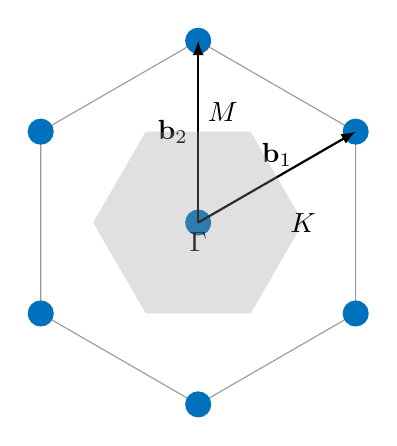
\begin{tikzpicture}[>=latex, scale=1.0, transform shape]
			% Draw the reciprocal lattice. Everything is multiplied by a factor of 2
			\draw[color=black!40!white] (2,{2/sqrt(3)}) node[circle,fill,color=myblue] {} -- (0,{4/sqrt(3)}) node[circle,fill,color=myblue] {} -- (-2,{2/sqrt(3)}) node[circle,fill,color=myblue] {} -- (-2,{-2/sqrt(3)}) node[circle,fill,color=myblue] {} -- (0,{-4/sqrt(3)}) node[circle,fill,color=myblue] {} -- (2,{-2/sqrt(3)}) node[circle,fill,color=myblue] {} -- cycle;
			\draw (0,0) node[circle,fill,color=myblue] {};
			\draw (0,0) node[black,below,opacity=1.0] {$\Gamma$};
			
			% Draw the reciprocal lattice vectors
			\draw[->, thick] (0,0) -- (2,{2/sqrt(3)}) node[midway, above] {$\vec{b}_1$};
			\draw[->, thick] (0,0) -- (0,{4/sqrt(3)}) node[midway, left] {$\vec{b}_2$};
			\draw[transparent] (0,0) -- (0,{4/sqrt(3)}) node[midway, above right, black, opacity=1.0] {$M$};
			
			% Highlight the BZ
			\fill[color=black!40!white,opacity=0.3] (4/3,0) node[black,opacity=1.0] {$K$} -- (2/3,{2/sqrt(3)}) -- (-2/3,{2/sqrt(3)}) -- (-4/3,0) -- (-2/3,{-2/sqrt(3)}) -- (2/3,{-2/sqrt(3)}) -- cycle;	
			\end{tikzpicture}
		\caption{Reciprocal lattice and Brillouin zone (highlighted in grey). $K$-, $\Gamma$- and $M$-points are also indicated.}
		\label{fig:graphene_BZ}
	\end{figure}
	
	Let's now construct the tight-binding Hamiltonian for an infinite system. Since we have two atoms in the elementary cell, the most general wavefunction obtained through Bloch's theorem will be
	\begin{equation}
		\Ket{\psi} = \sum_{R}e_{ikR}\Big\lbrace c_1\Ket{\phi_1(k,R)} + c_2\Ket{\phi_2(k,R)} \Big\rbrace
	\end{equation}
	where $\Ket{\phi_1(k,R)} = e^{ika_n}\Ket{R,n}$. Here, $R$ runs on the cell coordinates and $a_n$ is the coordinate of the $n$-th atom in the unit cell. Since we don't really need this information in order to write the tight-binding Hamiltonian, we don't care.
	
	Now, we want $\Ket{\psi}$ to be the solution of $H\Ket{\psi} = E(k)\Ket{\psi}$. By sandwiching this equation with $\Braket{\phi_1(k,R)}$ on the left (we'll avoid to write $k$ all around to keep things clean) we get
	\begin{equation}
		\Braket{\phi_1(R)|H|\psi(R)} = E\Braket{\phi_1(R)|\psi(R)} \approx Ec_1,
	\end{equation}
	where we have approximated the overlap matrix to the identity matrix. We'll say more words about this approximation later, but for the time being let's stick to this approach.
	
	So far, we've assumed nothing on the interactions. If we assume that the interactions are only of nearest-neighbor type, things simplify considerably. Namely, the sum $\sum_{R}$ now runs only on those $R$ which contain nearest-neighbor atoms of the one we are considering. Just to be even more clear, if we are calculating this at cell $\vec{R}=(0,0)$ for atom 1, then its nearest neighbors will be
	\begin{itemize}
		\item atom 2 in its own cell, at $\vec{R}=(0,0)$;
		\item atom 2 in the lower right cell, at $\vec{R} = -\vec{a}_2 = a\left(\frac{1}{2},-\frac{\sqrt{3}}{2}\right)$;
		\item atom 2 in the lower left cell, at $\vec{R} = -(\vec{a}_1+\vec{a}_2) = a\left(-\frac{1}{2},-\frac{\sqrt{3}}{2}\right)$.
	\end{itemize}
	So, in the end you will get:
	\begin{align}
		Ec_1
		&= c_1\underbrace{\Braket{\phi_1(0,0)|H|\phi_1(0,0)}}_{\varepsilon} + c_2\underbrace{\Braket{\phi_1(0,0)|H|\phi_2(0,0)}}_{-t} \nonumber \\
		&+ e^{ia(k_x\frac{1}{2}-k_y\frac{\sqrt{3}}{2})}c_2\underbrace{\Braket{\phi_1(0,0)|H|\phi_2(-\vec{a}_2)}}_{-t} \nonumber \\
		&+ e^{-ia(k_x\frac{1}{2}+k_y\frac{\sqrt{3}}{2})}c_2\underbrace{\Braket{\phi_1(0,0)|H|\phi_2(-\vec{a}_1-\vec{a}_2)}}_{-t} \nonumber \\
		&= c_1\varepsilon -tc_2\left(1 + e^{i\frac{a}{2}(k_x-\sqrt{3}k_y)} + e^{-i\frac{a}{2}(k_x+\sqrt{3}k_y)}\right) \nonumber \\
		&\doteqdot c_1\varepsilon -tc_2f(\vec{k}).
	\end{align}
	Similarly, by taking into account the other orbital, you get
	\begin{equation}
		Ec_2 = c_2\varepsilon -tc_1f^*(\vec{k}).
	\end{equation}
	
	In matrix form, these two equations will read as
	\begin{equation}
		\left(
		\begin{array}{cc}
			\varepsilon - E & -tf(\vec{k}) \\
			-tf^*(\vec{k}) & \varepsilon - E
		\end{array}
		\right)
		\left(
			\begin{array}{c}
				c_1 \\
				c_2			
			\end{array}
		\right)
		= 0.
	\end{equation}
	
	By setting the determinant to zero and playing a bit with sines and cosines, you finally get the expression
	\begin{equation}
		\boxed{E(\vec{k}) = \varepsilon \pm t\sqrt{1 + 4\cos\left(\frac{k_xa}{2}\right)\cos\left(\frac{\sqrt{3}k_ya}{2}\right) + 4\cos^2\left(\frac{k_xa}{2}\right)}}.
	\end{equation}
	
	As you see, we get two \emph{symmetric} bands above and below $\varepsilon$. This is usually not the case, since the overlap matrix in general is different from the identity. Taking this fact into account, the dispersion would be given by
	\begin{equation}
		E(\vec{k}) = \frac{\varepsilon \pm t\sqrt{1 + 4\cos\left(\frac{k_xa}{2}\right)\cos\left(\frac{\sqrt{3}k_ya}{2}\right) + 4\cos^2\left(\frac{k_xa}{2}\right)}}{1 \pm s\sqrt{1 + 4\cos\left(\frac{k_xa}{2}\right)\cos\left(\frac{\sqrt{3}k_ya}{2}\right) + 4\cos^2\left(\frac{k_xa}{2}\right)}},
	\end{equation}
	which is what you usually find in books, and where $s$ is the overlap parameter. For the present discussion, let's stick to the simplified symmetric-bands model.
	
	The eigenfunctions of this Hamiltonian, given its symmetry, will be
	\begin{equation}
		\frac{1}{\sqrt{2}}
		\left(
			\begin{array}{c}
				\frac{f(\vec{k})}{|f(\vec{k})|} \\
				1
			\end{array}
		\right)
		\qquad\text{and}\qquad
		\frac{1}{\sqrt{2}}
		\left(
			\begin{array}{c}
				-\frac{f(\vec{k})}{|f(\vec{k})|} \\
				1
			\end{array}
		\right).
	\end{equation}
	
	If you plot this energy as a function of the components of $E(\vec{k})$, you will get the results sown in Figure \ref{fig:E_of_k} and \ref{fig:E_of_k_over_BZ}.
	\begin{figure}[H]
		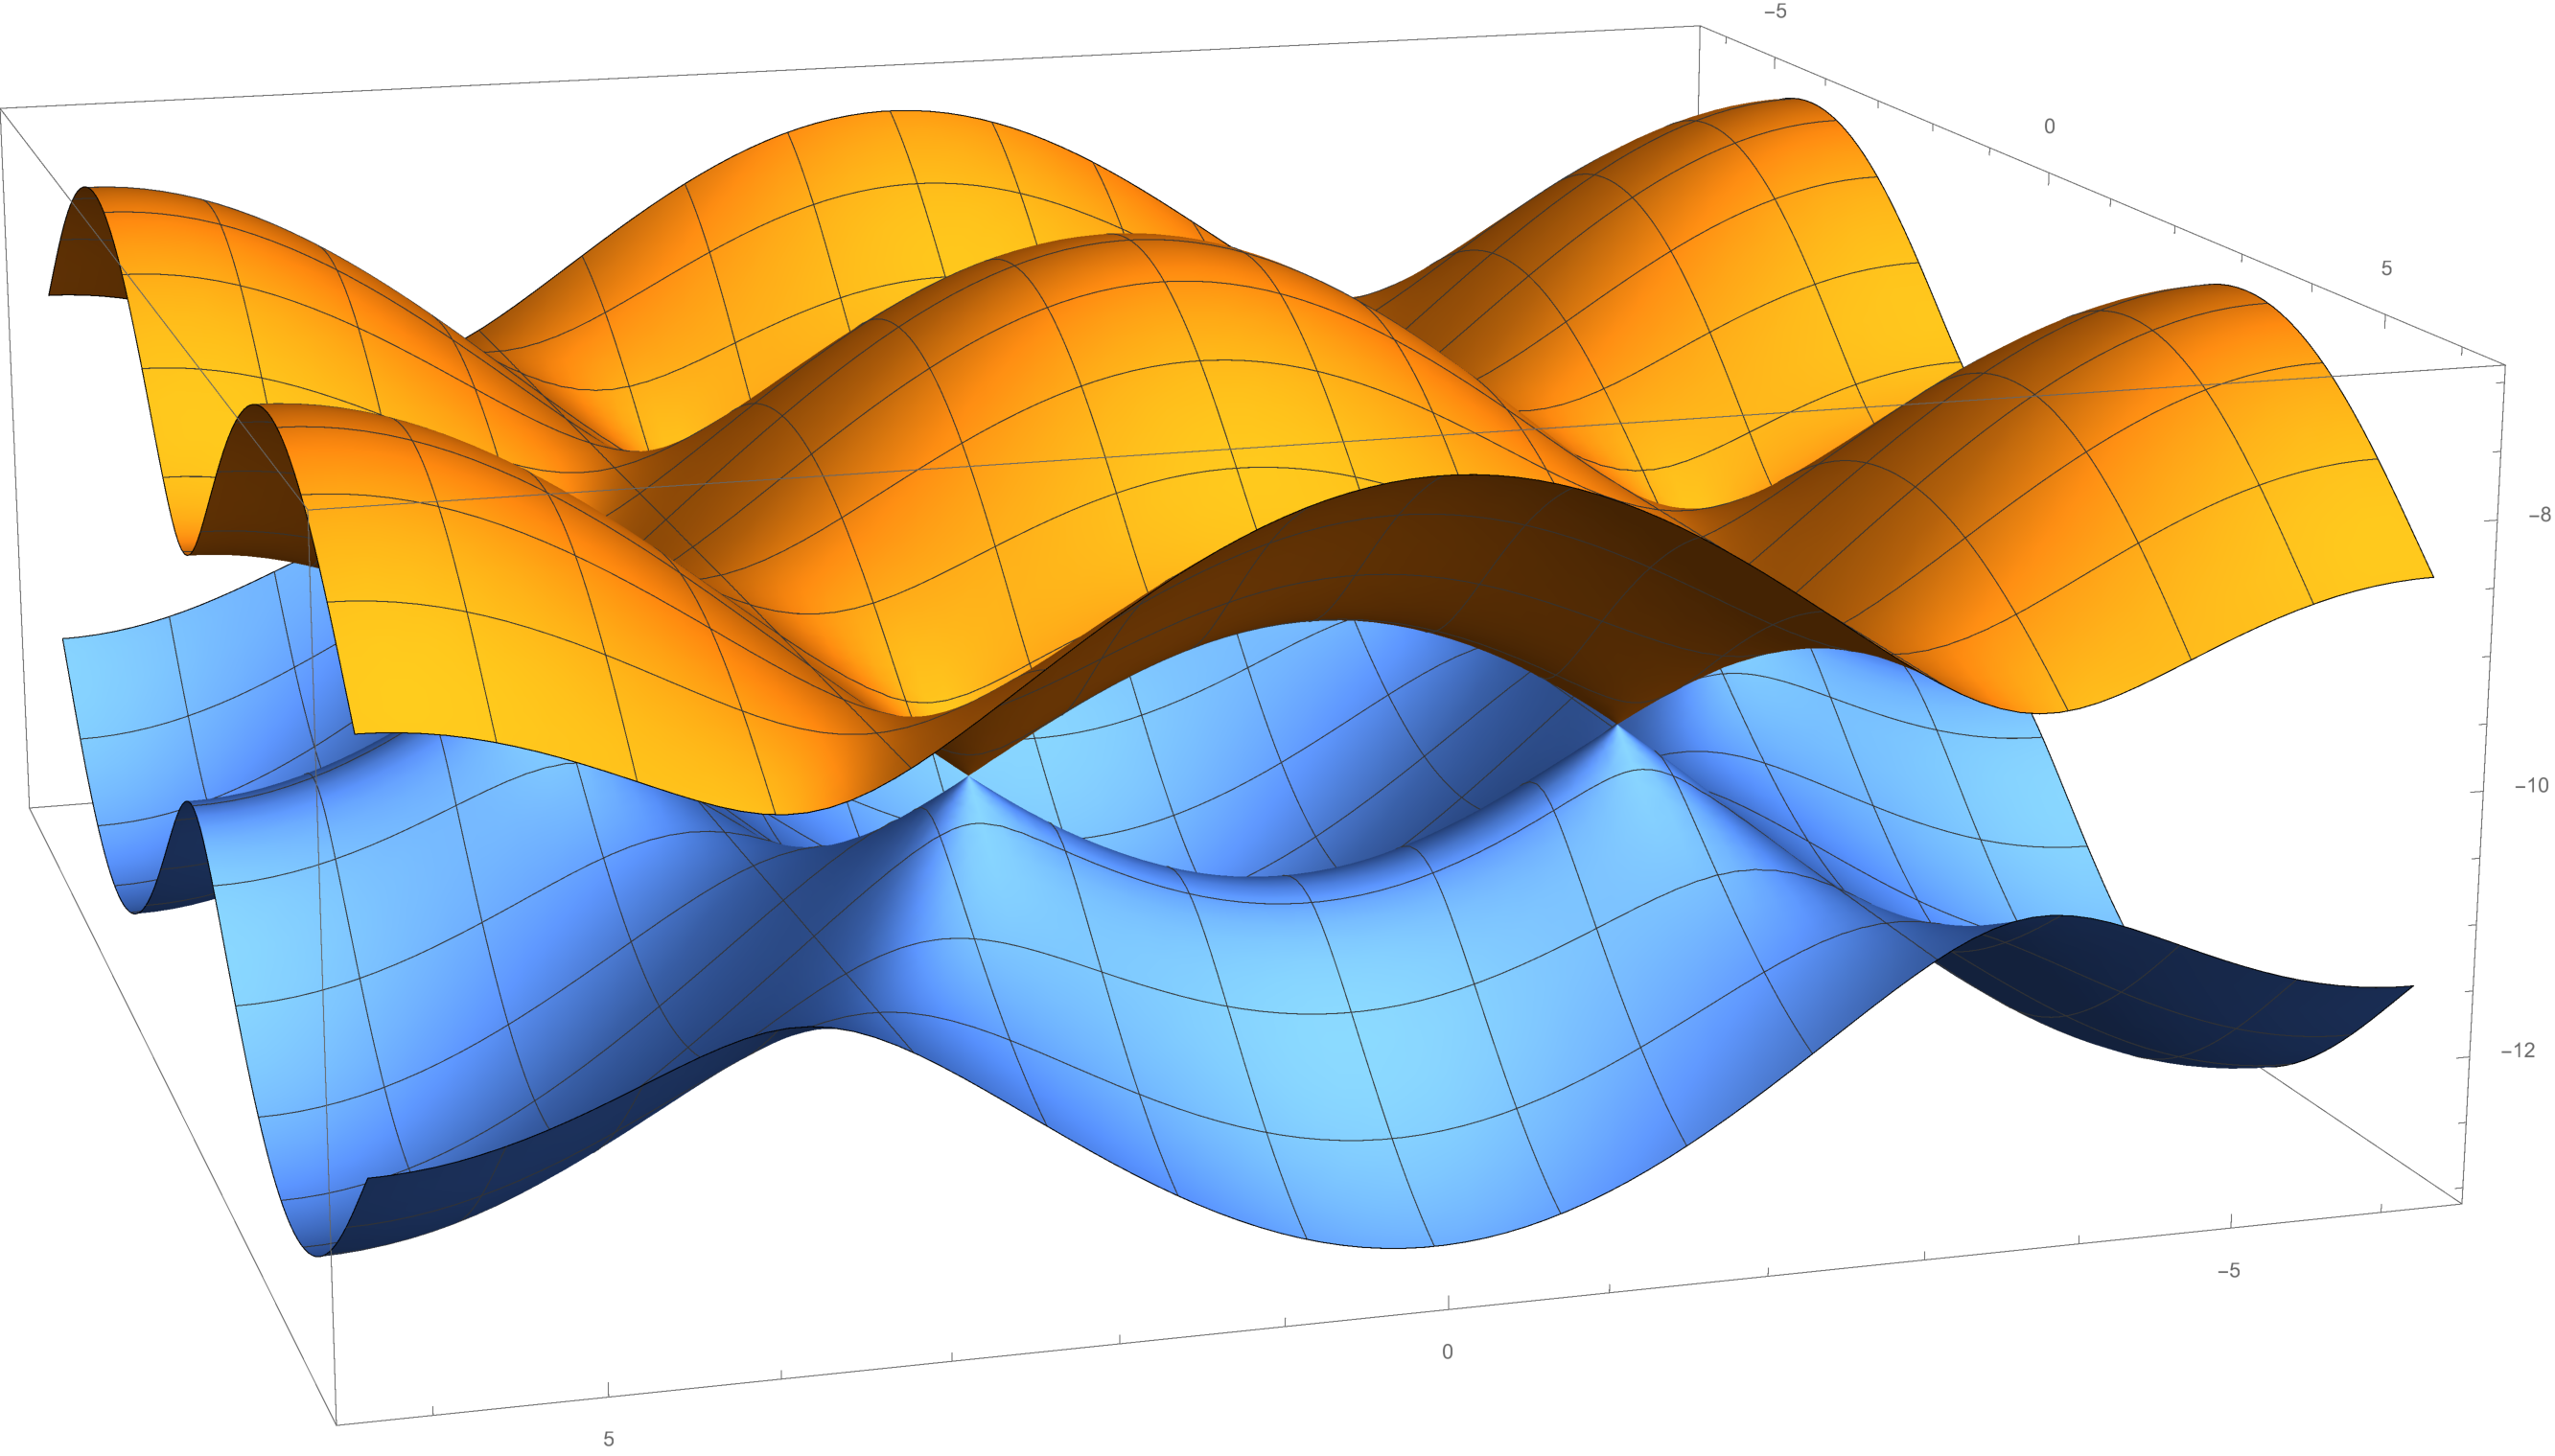
\includegraphics[width=\textwidth]{E_of_k}
		\caption{Plot of $E(\vec{k})$ over a $k_x-k_y$ plane which is \emph{larger} than the Brillouin zone. The values used are $\varepsilon = -10$, $t=1$ and $a=1$.}
		\label{fig:E_of_k}
	\end{figure}
		\begin{figure}[H]
		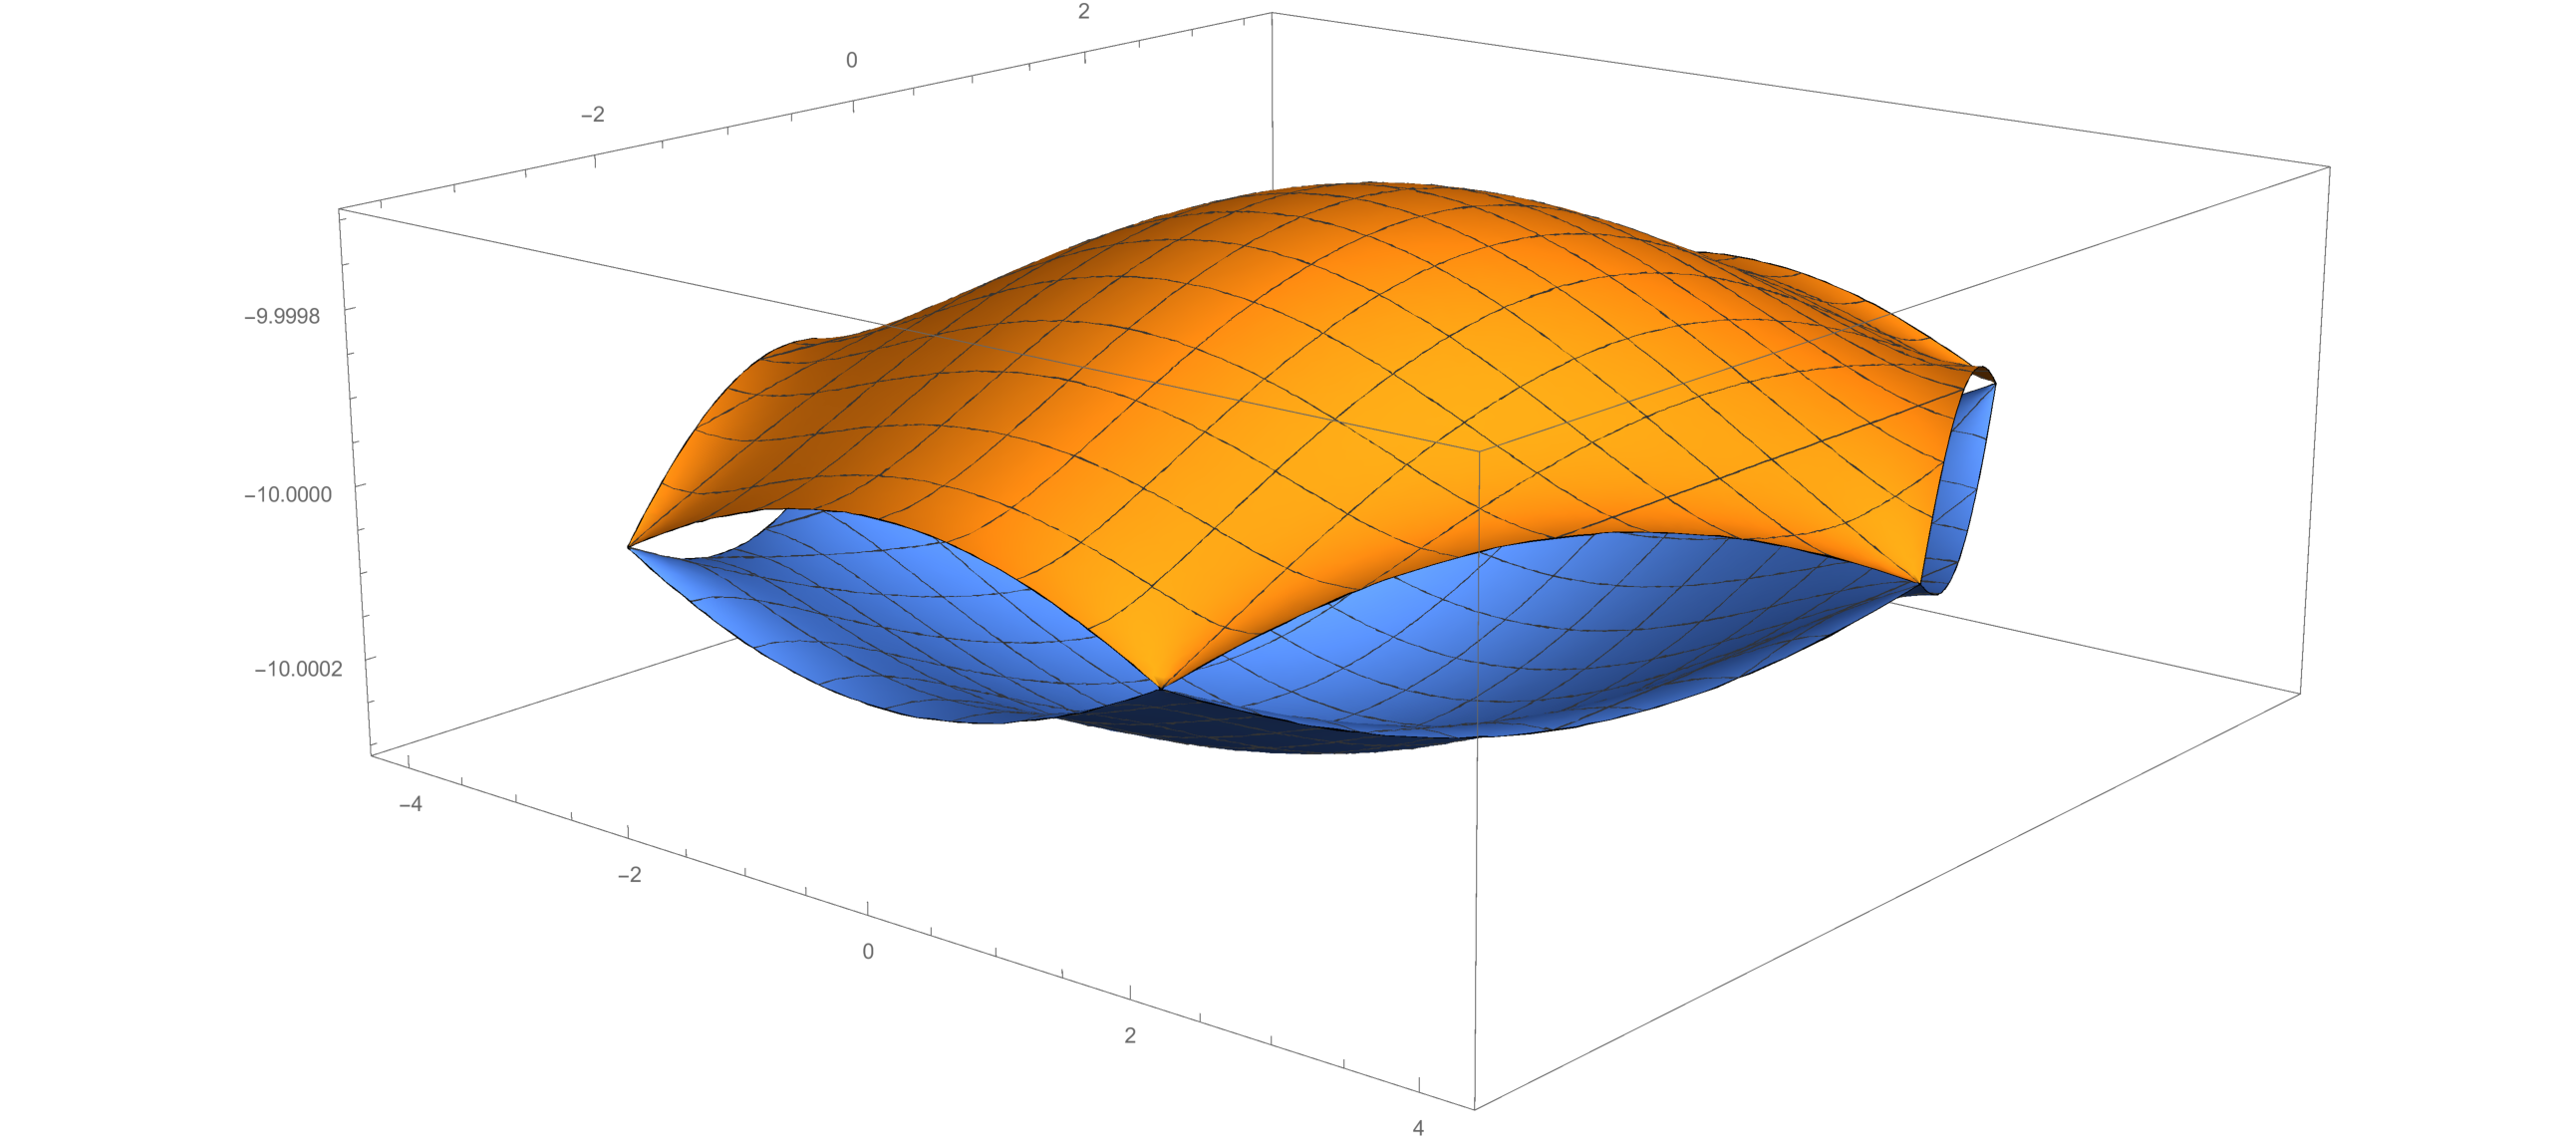
\includegraphics[width=\textwidth]{E_of_k_over_BZ}
		\caption{Plot of $E(\vec{k})$ over the Brillouin zone. The values used are $\varepsilon = -10$, $t=1$ and $a=1$.}
		\label{fig:E_of_k_over_BZ}
	\end{figure}
	
	In Figure \ref{fig:E_of_k}, the presence of the Dirac cones for $E-\varepsilon=0$ is evident (at K points); you can also see the presence of saddle points (at M points).
	
	Now, starting from this result, we can compute numerically the density of states. The trick is simply to sample the energy over a large number of points in the Brillouin zone (the energy over the BZ looks like Figure \ref{fig:E_of_k_over_BZ}). Then, you can just do an histogram normalized as a PDF to get the density of states. Furthermore, in this case the two bands are symmetric so we can just sample one band and then add the same samples with a minus sign in front.
	
	With \Mathematica, these operations are achieved via the 5-lines code in the attached \texttt{DOS\_Simulation.nb}. The result is shown in Figure \ref{fig:DOS_Mathematica}.
	
	With the chosen parameters, we sampled over $\SI{3.5E6}{}$ energy values in the Brillouin zone and we got $300$ bins in the final histogram.
	
	\begin{figure}[H]
		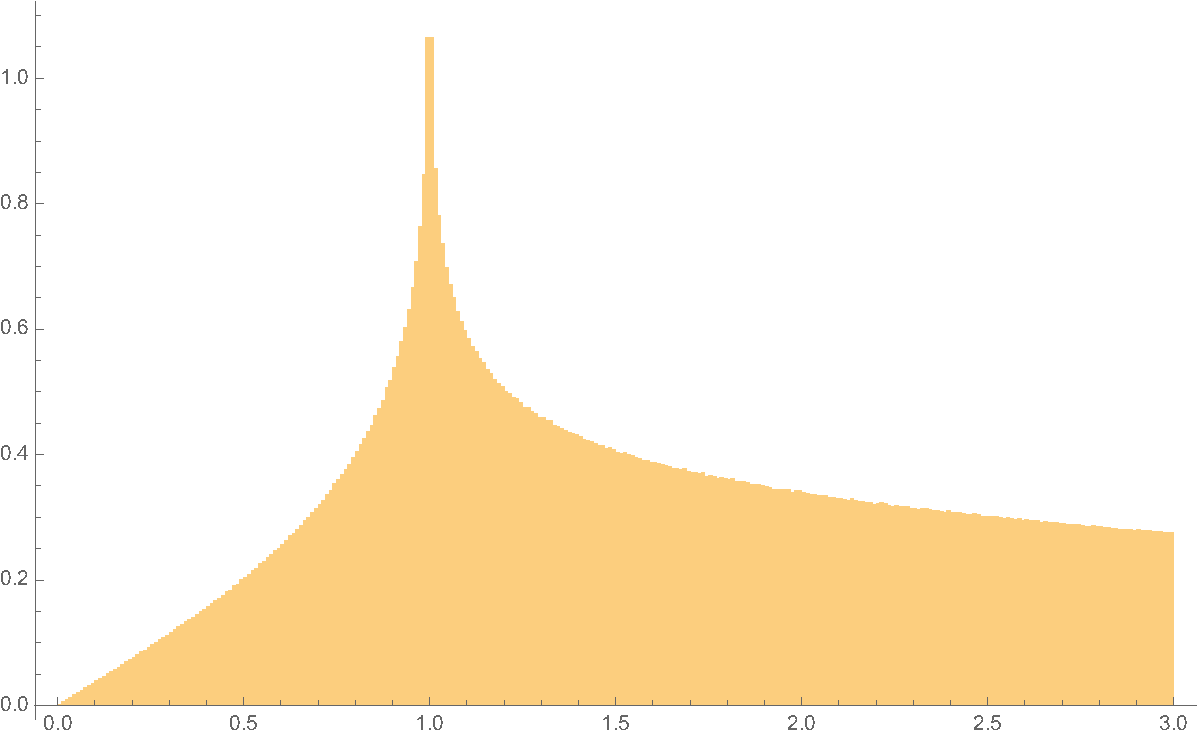
\includegraphics[width=\textwidth]{DOS}
		\caption{Plot of the positive-energies part of the density of states. The values used are $\varepsilon = 0$ (which doesn't matter, it's just the scale of our energy), $t=1$ and $a=1$. The histogram is normalized as a PDF, but here we still have to add the negative-energies part; so, upon renormalizing, the values on the vertical axis of the DOS will be half of these ones (look at Figure \ref{fig:DOS_and_fits}).}
		\label{fig:DOS_Mathematica}
	\end{figure}
	
	Then, we imported in \MATLAB\ the samples generated with \Mathematica, in order to do some further manipulations. All the manipulations were done automatically via the attached script \texttt{DOS\_FIT.m}, which took care of including the mirror branch of the DOS and did some fits. The results are shown in Figure \ref{fig:DOS_and_fits}. The energy is plotted in units of $t$, so for e.g. $t \sim \SI{2.5}{e\volt}$ the energy scale will go from $-\SI{7.5}{e\volt}$ to $\SI{7.5}{e\volt}$.
	
	\begin{figure}[H]
		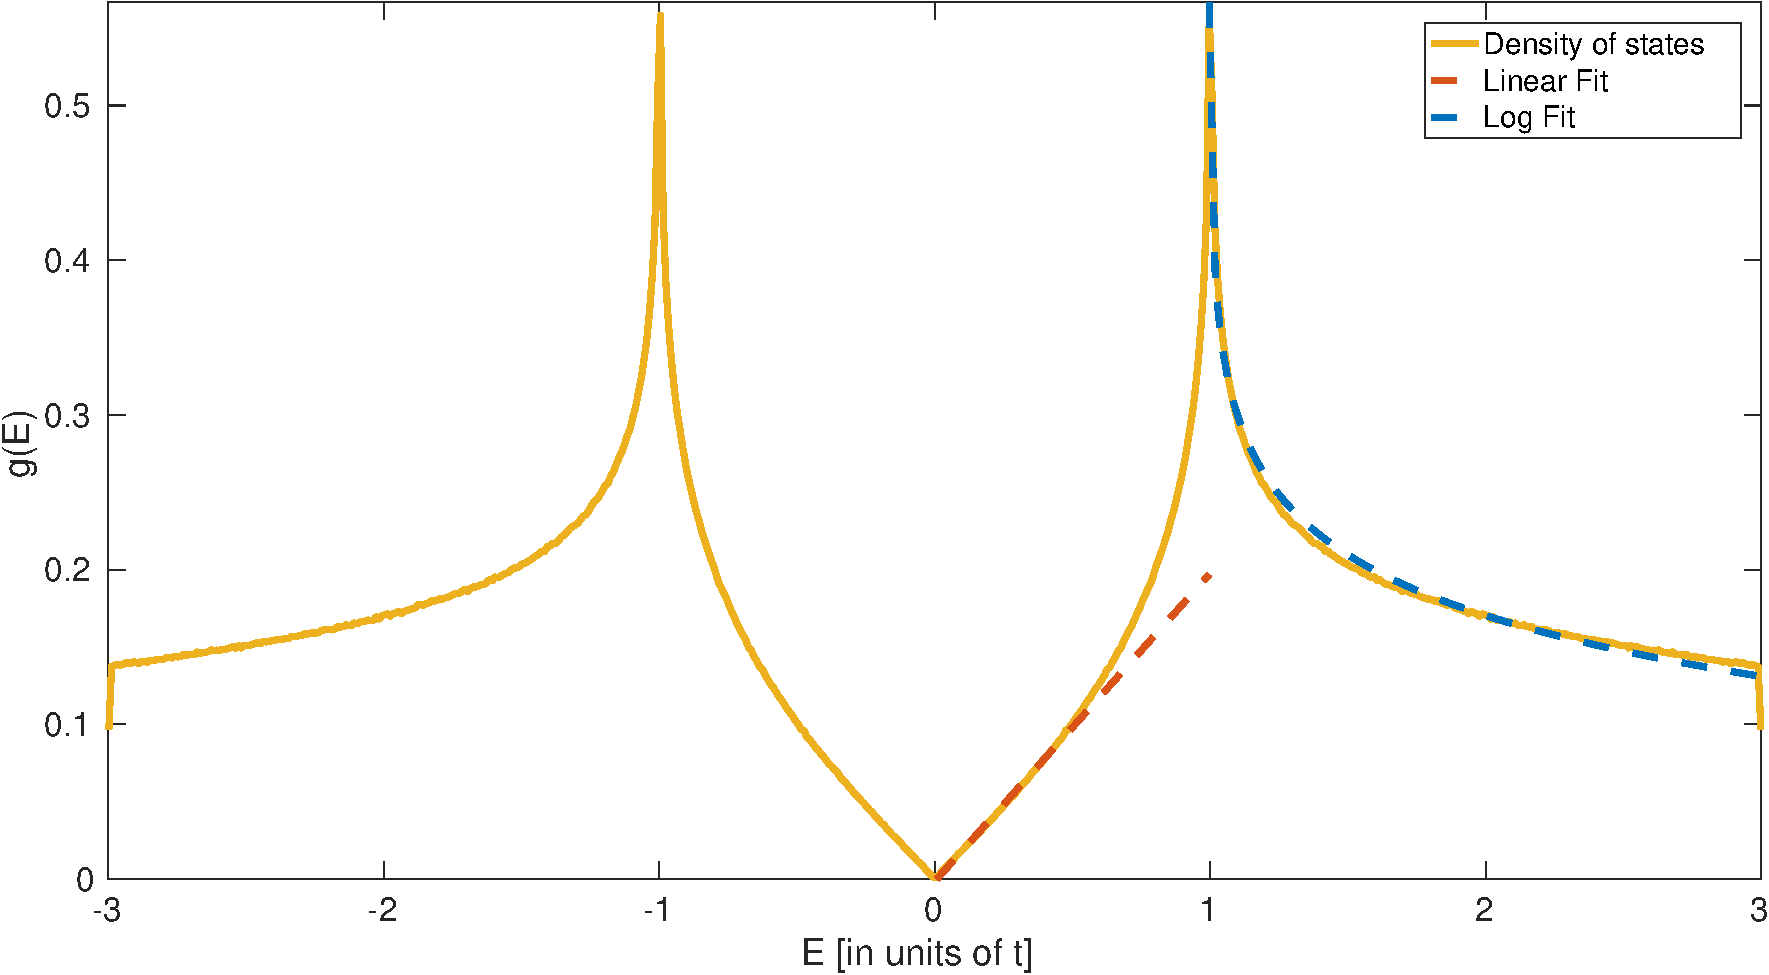
\includegraphics[width=\textwidth]{DOS_and_fits}
		\caption{Complete and properly normalized DOS with a linear and a log fit.}
		\label{fig:DOS_and_fits}
	\end{figure}
	
	As you see, the DOS goes to zero in correspondence of the K-points, while it diverges logarithmically in correspondence of the M-points (which are saddle points of the energy). In order to formally verify that the M-points are indeed saddle points, we calculated the Hessian matrix in those points; as expected, their eigenvalues have different signs. These calculations are not reported here but are contained in \texttt{A\_Hessian.nb}.

\end{proof}



\begin{problem}[B4. Armchair carbon nanotube]
	Refer to the assignment paper for the text of the problem.
\end{problem}
\begin{proof}

%%% YUSUF DISCUSSION STARTS HERE

Consider an armchair nanotube with its axis parallel to the x-direction of cartesian the  coordinate. Thus, in the unrolled state, in this case a zigzag nanoribon, has a finite dimension (depending on the tube diameter of interest) along y-direction. The periodic  boundary conditions required that the energy is quantized along the y-component of the momentum in the reciprocal space.

We defined the primitive vectors of graphene in the following way:
\begin{equation}
		\vec{a}_1 = \frac{a}{2} (1,\sqrt(3))
		\qquad\text{and}\qquad
		\vec{a}_2 = \frac{a}{2}\left(-1,\sqrt{3}\right).
	\end{equation}
    Here we define a chiral vector $\vec{C_h}$ which is perpendicular to the axis of the tube (along y-axis by our construction) and another vector $\vec{T}$, called the translational vector, along the axis of the tube that describes the periodicity in the infinite direction as follows:
    \begin{equation}
    \vec{C_h}=N(\vec{a_1}+\vec{a_2})
        \qquad\text{and}\qquad
        \vec{T}=\vec{a_1}-\vec{a_2}
    \end{equation}
    where N is an integer. 
The smallest unit of the armchair nanotube (NT) is the rectangle enclosed by the  $\vec{C_h}$ and $\vec{T}$ when N is set to 1. Thus, the value of N defines the size of the NT. The lattice parameter of the nanotube is the length of $\vec{T}$. In addition, $\vec{T}$ defines the one dimensional unit cell of the NT. And the corresponding one dimensional reciprocal lattice vector is $\vec{T^\prime}=\frac{2\pi}{a}(0,1)=$. Therefore, the 1-D Brillouin zone is in the interval $[-\frac{\pi}{a},\frac{\pi}{a}]$

%%%% MATTEO STUFF BEGINS HERE
	
	The text of the problem describes the construction of a zig-zag nanotube, but then it says that it's an armchair nanotube. For consistency with the nomenclature found all along in the literature, we consider in this solution what is usually called an armchair nanotube, i.e. the object constructed following the guidelines in Figure \ref{fig:carbon_nanotube_armchair}.
	
	The length of the circumference of a nanotube is usually described by a so-called \emph{wrapping vector} (or \emph{curling vector}) $\vec{w} = N\vec{a}_1+M\vec{a}_2$, where $\vec{a}_1$ and $\vec{a}_2$ are the symmetric lattice basis vector, depicted for reference in Figure \ref{fig:carbon_nanotube_armchair}. $N$ and $M$ are chosen in such a way that $\vec{w}$ is perpendicular to the axis of the nanotube, so the nanotube itself can be completely characterized by the pair $(N,M)$. In our case $N=M$, so the nanotube is of type $(N,N)$\footnote{$(N,N)$ is the standard notation that indicated an armchair-type nanotube.}. Notice that, given its definition, the length of $\vec{w}$ coincides with the length of the circumference of the nanotube.
	
	As shown in Figure \ref{fig:carbon_nanotube_armchair}, now the unit cell is a ring of width $a$ and circumference $||\vec{w}||$; this means that in general the unit cell of an armchair nanotube contains $4N$ atoms and the resulting tight-binding matrix will have dimensions $4N\times4N$.
	
	
	\begin{figure}[H]
		\centering
		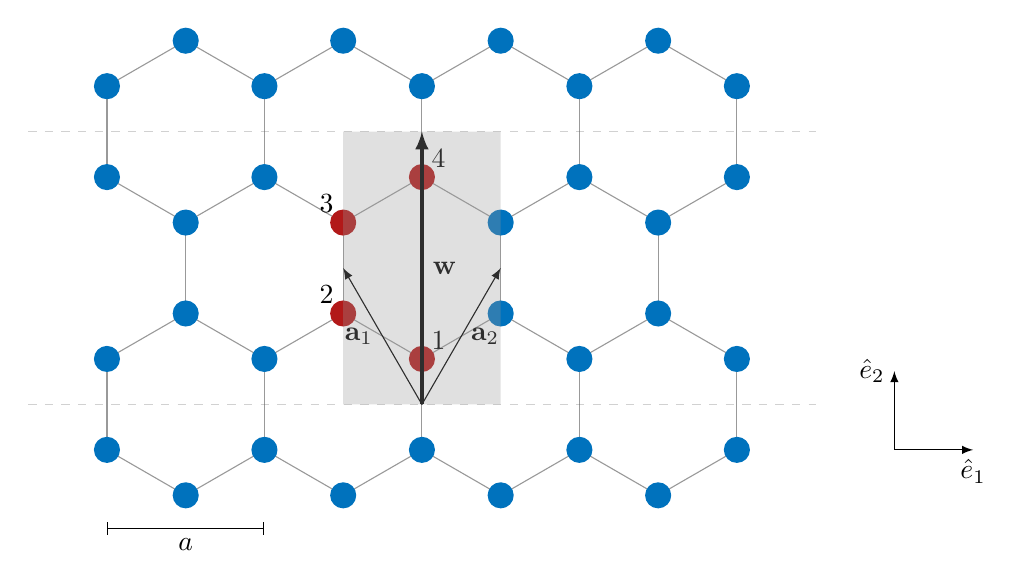
\begin{tikzpicture}[>=latex, scale=1.0, transform shape]
			% Draw the horizontal zig-zag lines and some dots. a=2
			\draw[color=black!40!white] (0,0) -- (1,-{sqrt(3)/3}) node[circle,fill,color=myblue] {} -- (2,0) -- (3,-{sqrt(3)/3}) node[circle,fill,color=myblue] {} -- (4,0) -- (5,-{sqrt(3)/3}) node[circle,fill,color=myblue] {} -- (6,0) -- (7, -{sqrt(3)/3}) node[circle,fill,color=myblue] {} -- (8,0);
			\draw[color=black!40!white] (0,{2*sqrt(3)/3}) -- (1,{sqrt(3)}) -- (2,{2*sqrt(3)/3}) -- (3,{sqrt(3)}) -- (4,{2*sqrt(3)/3}) -- (5,{sqrt(3)}) -- (6,{2*sqrt(3)/3}) -- (7,{sqrt(3)}) -- (8,{2*sqrt(3)/3});
			\draw[color=black!40!white] (0,{2*sqrt(3)}) -- (1,{5*sqrt(3)/3}) -- (2,{2*sqrt(3)}) -- (3,{5*sqrt(3)/3}) -- (4,{2*sqrt(3)}) -- (5,{5*sqrt(3)/3}) -- (6,{2*sqrt(3)}) -- (7,{5*sqrt(3)/3}) -- (8,{2*sqrt(3)});
			\draw[color=black!40!white] (0,{8*sqrt(3)/3}) -- (1,{3*sqrt(3)}) node[circle,fill,color=myblue] {} -- (2,{8*sqrt(3)/3}) -- (3,{3*sqrt(3)}) node[circle,fill,color=myblue] {} -- (4,{8*sqrt(3)/3}) -- (5,{3*sqrt(3)}) node[circle,fill,color=myblue] {} -- (6,{8*sqrt(3)/3}) -- (7,{3*sqrt(3)}) node[circle,fill,color=myblue] {} -- (8,{8*sqrt(3)/3});
			
			% Draw the vertical connecting lines and the circles
			\draw[color=black!40!white] (0,0) node[circle,fill,color=myblue] {} -- (0,{2*sqrt(3)/3}) node[circle,fill,color=myblue] {};
			\draw[color=black!40!white] (2,0) node[circle,fill,color=myblue] {} -- (2,{2*sqrt(3)/3}) node[circle,fill,color=myblue] {};
			\draw[color=black!40!white] (4,0) node[circle,fill,color=myblue] {} -- (4,{2*sqrt(3)/3}) node[circle,fill,color=myred] {};
			\draw[color=black!40!white] (6,0) node[circle,fill,color=myblue] {} -- (6,{2*sqrt(3)/3}) node[circle,fill,color=myblue] {};
			\draw[color=black!40!white] (8,0) node[circle,fill,color=myblue] {} -- (8,{2*sqrt(3)/3}) node[circle,fill,color=myblue] {};
			\draw[color=black!40!white] (1,{sqrt(3)}) node[circle,fill,color=myblue] {} -- (1,{5*sqrt(3)/3}) node[circle,fill,color=myblue] {};
			\draw[color=black!40!white] (3,{sqrt(3)}) node[circle,fill,color=myred] {} -- (3,{5*sqrt(3)/3}) node[circle,fill,color=myred] {};
			\draw[color=black!40!white] (5,{sqrt(3)}) node[circle,fill,color=myblue] {} -- (5,{5*sqrt(3)/3}) node[circle,fill,color=myblue] {};
			\draw[color=black!40!white] (7,{sqrt(3)}) node[circle,fill,color=myblue] {} -- (7,{5*sqrt(3)/3}) node[circle,fill,color=myblue] {};
			\draw[color=black!40!white] (0,{2*sqrt(3)}) node[circle,fill,color=myblue] {} -- (0,{8*sqrt(3)/3}) node[circle,fill,color=myblue] {};
			\draw[color=black!40!white] (2,{2*sqrt(3)}) node[circle,fill,color=myblue] {} -- (2,{8*sqrt(3)/3}) node[circle,fill,color=myblue] {};
			\draw[color=black!40!white] (4,{2*sqrt(3)}) node[circle,fill,color=myred] {} -- (4,{8*sqrt(3)/3}) node[circle,fill,color=myblue] {};
			\draw[color=black!40!white] (6,{2*sqrt(3)}) node[circle,fill,color=myblue] {} -- (6,{8*sqrt(3)/3}) node[circle,fill,color=myblue] {};
			\draw[color=black!40!white] (8,{2*sqrt(3)}) node[circle,fill,color=myblue] {} -- (8,{8*sqrt(3)/3}) node[circle,fill,color=myblue] {};

			% Draw the coordinate system
			\draw[->] (10,0) -- (11,0) node[below] {$\hat{e}_1$};
			\draw[->] (10,0) -- (10,1) node[left] {$\hat{e}_2$};
			
			% Draw the basis vectors and the wrapping vector
			\draw[->] (4,{sqrt(3)/3}) -- (3,{sqrt(3)+sqrt(3)/3}) node[midway, left] {$\vec{a}_1$};
			\draw[->] (4,{sqrt(3)/3}) -- (5,{sqrt(3)+sqrt(3)/3}) node[midway, right] {$\vec{a}_2$};
			\draw[->, very thick] (4,{sqrt(3)/3}) -- (4,{2*sqrt(3)+sqrt(3)/3}) node[midway, right] {$\vec{w}$};
			
			% Label the atoms
			\draw (4,{2*sqrt(3)/3}) node[above right] {$1$};
			\draw (3,{sqrt(3)}) node[above left] {$2$};
			\draw (3,{5*sqrt(3)/3}) node[above left] {$3$};
			\draw (4,{2*sqrt(3)}) node[above right] {$4$};
			
			% Highlight the elementary cell
			\fill[color=black!40!white,opacity=0.3] (4,{sqrt(3)/3}) -- (5,{sqrt(3)/3}) -- (5,{2*sqrt(3)+sqrt(3)/3}) -- (3,{2*sqrt(3)+sqrt(3)/3}) -- (3,{sqrt(3)/3}) -- cycle;
			
			% Draw the cutting lines
			\draw[color=black!60!white,opacity=0.3, dashed] (-1,{sqrt(3)/3}) -- (9,{sqrt(3)/3});
			\draw[color=black!60!white,opacity=0.3, dashed] (-1,{2*sqrt(3)+sqrt(3)/3}) -- (9,{2*sqrt(3)+sqrt(3)/3});
		
			% Put some units
			\draw[|-|] (0,-1) -- (2,-1) node[midway, below] {$a$};
		\end{tikzpicture}
		\caption{Construction of an armchair nanotube for $N=1$ ($(1,1)$ nanotube). The graphene sheet is cut along the horizontal dashed lines; the stripe obtained in this way extends in infinite direction along $\hat{e}_1$, while it covers two elementary graphene cells in the $\hat{e}_2$ direction. In other words, it's basically a zig-zag ribbon. Then the ribbon is folded along the zig-zag edges, in such a way that atom $1$ and atom $4$ are now first nearest neighbors and $\hat{e}_1$ is the axis of the so-obtained infinite cylinder.}
		\label{fig:carbon_nanotube_armchair}
	\end{figure}
	
	To construct the matrix, we start from the case $N=1$. Following a procedure which is completely similar to the one described in problem \ref{pro:A}, we obtain the tight-binding matrix in the basis $\Ket{R,n}$\footnote{Where now $n$ goes from $1$ to $4$ because we have $4$ atoms in the unit cell.}:
	\begin{equation}
		H = 
		\left(
			\begin{array}{cccc}
			\varepsilon & -tf(\vec{k}) & 0 & -tg^*(\vec{k)} \\
			-tf^*(\vec{k)} & \varepsilon & -tg(\vec{k}) & 0  \\
			0 & -tg^*(\vec{k)} & \varepsilon & -tf(\vec{k}) \\
			-tg(\vec{k}) & 0 & -tf^*(\vec{k)} & \varepsilon  \\
			\end{array}
		\right)
	\end{equation}
	where
	\begin{equation}
		f(\vec{k}) = 2\cos\left(\frac{k_xa}{2}\right)e^{i\frac{k_ya}{2\sqrt{3}}}
		\qquad\text{and}\qquad
		g(\vec{k}) = e^{i\frac{k_ya}{\sqrt{3}}}.
	\end{equation}
	
	The extension of this matrix for $N>1$ is trivial; it will just be a matrix with diagonal elements equal to $\varepsilon$, upper diagonal with alternating $-tf(\vec{k})$ and $-tg(\vec{k})$, and upper right corner equal to $-tg^*(\vec{k})$ to make the Hamiltonian periodic. Then, the lower triangle of the matrix is found by complex-conjugating in order to make the Hamiltonian hermitian.
	
	The big difference with the graphene case, apart from the increasing dimension of the matrix, is in the shape of the Brillouin zone. In fact, since the system is basically unidimensional (along $\hat{e}_{1}$), you expect that the Brillouin zone will be unidimensional. This is in fact the case, and the BZ extends from $k_x = -\pi/a$ to $k_x = \pi/a$. So then, what is the role of $k_y$? Where does it enter?
	
	The system is, strictly speaking, infinite also along the circumference\footnote{A bug that moves along the circumference will never escape from the surface of the tube!}, but \emph{we made it infinite} by imposing periodic boundary conditions. This means that not every wave can run along the circumference; only waves that respect the PBC's are allowed. This in turn translates into a condition over the set of the allowed $k_y$, that now is no more $\mathbb{R}$ but it's a set of discrete, quantized values. Namely, the allowed $k_y$ values are
	\begin{equation}
		k_y = \frac{2\pi}{a\sqrt{3}}\left(\frac{m}{N}\right), 
		\qquad -N \leq m \leq N.
	\end{equation}
	
	So, for each value of $k_y$, we have an energy matrix that is only function of $k_x$ and that we have to diagonalize in order to find the dispersion law. Since this job becomes analytically harder and harder for increasing values of $N$, we wrote a routine (both in \Mathematica\ and Fortran) that builds the required matrix and diagonalizes it numerically for different values of $k_y$.

	\begin{figure}[H]
		\centering
		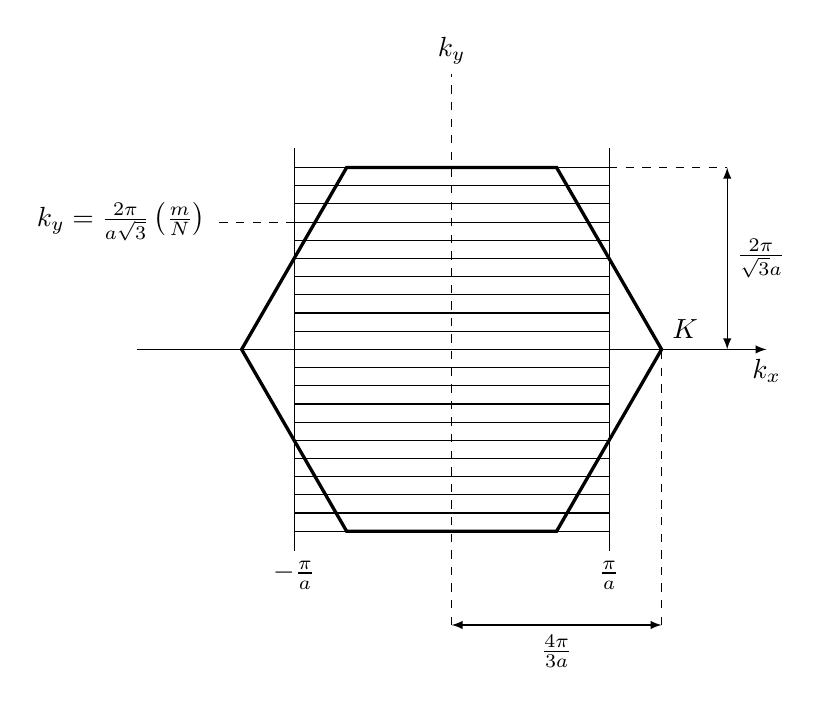
\begin{tikzpicture}[>=latex, scale=1.0, transform shape]
			% Draw the axes
			\draw[->] (-4,0) -- (4,0) node[below] {$k_x$};
			\draw[dashed] (0,-3.5) -- (0,3.5) node[above] {$k_y$};
			
			% Draw the graphene BZ
			\draw[color=black, very thick] (8/3,0) node[black,opacity=1.0, above right] {$K$} -- (4/3,{4/sqrt(3)}) -- (-4/3,{4/sqrt(3)}) -- (-8/3,0) -- (-4/3,{-4/sqrt(3)}) -- (4/3,{-4/sqrt(3)}) -- cycle;
			
			% Draw the vertical lines
			\draw[color=black] (2,{-4/sqrt(3)-0.25}) node[below] {$\frac{\pi}{a}$} -- (2,{4/sqrt(3)+0.25});
			\draw[color=black] (-2,{-4/sqrt(3)-0.25}) node[below] {$-\frac{\pi}{a}$} -- (-2,{4/sqrt(3)+0.25});
			
			% Draw the ky lines
			\foreach \m in {-10,...,10}
			{
				\draw[color=black] (-2,{4/sqrt(3)/10*\m}) -- (2,{4/sqrt(3)/10*\m});
			}
			
			% Draw units and stuff
			\draw[dashed] (8/3,-3.5) -- (8/3,0);
			\draw[<->] (0,-3.5) -- (8/3,-3.5) node[midway,below] {$\frac{4\pi}{3a}$};
			\draw[dashed] (-2,{4/sqrt(3)/10*7}) -- (-3,{4/sqrt(3)/10*7}) node[left] {$k_y = \frac{2\pi}{a\sqrt{3}}\left(\frac{m}{N}\right)$};
			\draw[dashed] (2,{4/sqrt(3)}) -- (3.5,{4/sqrt(3)});
			\draw[<->] (3.5,0) -- (3.5,{4/sqrt(3)}) node[midway,right] {$\frac{2\pi}{\sqrt{3}a}$};
			
		\end{tikzpicture}
		\caption{1D Brillouin zone of a $(10,10)$ armchair carbon nanotube on top of the 2D Brillouin zone of the graphene.}
		\label{fig:armchair_BZ}
	\end{figure}
	
	The number of bands is $4N$ (since the matrix is $4N\times4N$), which is $40$ for $N=10$, but in Figure \ref{fig:B_E_of_k} only $22$ dispersion lines appear ($11$ above and $11$ below). This is because the bands corresponding to $-m$ and to $m$ are \emph{degenerate}, apart from the ones for $m=0$ and $m=\pm N$. In fact, you see that $2\cdot(9\cdot2+2\cdot1)=40$\footnote{Out of $11$ bands in each half plane of Figure \ref{fig:B_E_of_k}, $9$ of them are double-degenerate and $2$ of them are single-degenerate.}. The explanation of this fact can be understood in two ways. The first argument is that we are squeezing $2N$ graphene cells into one armchair unit cell, so a two-fold degeneracy appears. The second argument is that we are basically taking $k_y$-fixed \emph{slices} of the graphene dispersion (the one plotted in Figure \ref{fig:E_of_k}) along $k_x$; from the figure, you see that $k_y$ and $-k_y$ correspond to the same value of the energy, except for $k_y=0$ (i.e., $m=0$) and $k_y = \pm\frac{2\pi}{a\sqrt{3}}$ (i.e., $m = \pm N$).
	
	The second argument is useful because it automatically gives the behavior of the system from $N\to\infty$: we take slices of the graphene dispersion for finer and finer values of $k_y$, to the limit in which we take slices at every $k_y \in \mathbb{R}$. In this limit, the nanotube is basically indistinguishable from the graphene! This matches our physical intuition, since an infinite cylinder with infinite radius is basically indistinguishable from an infinite 2D plane.
	
	\begin{figure}[H]
		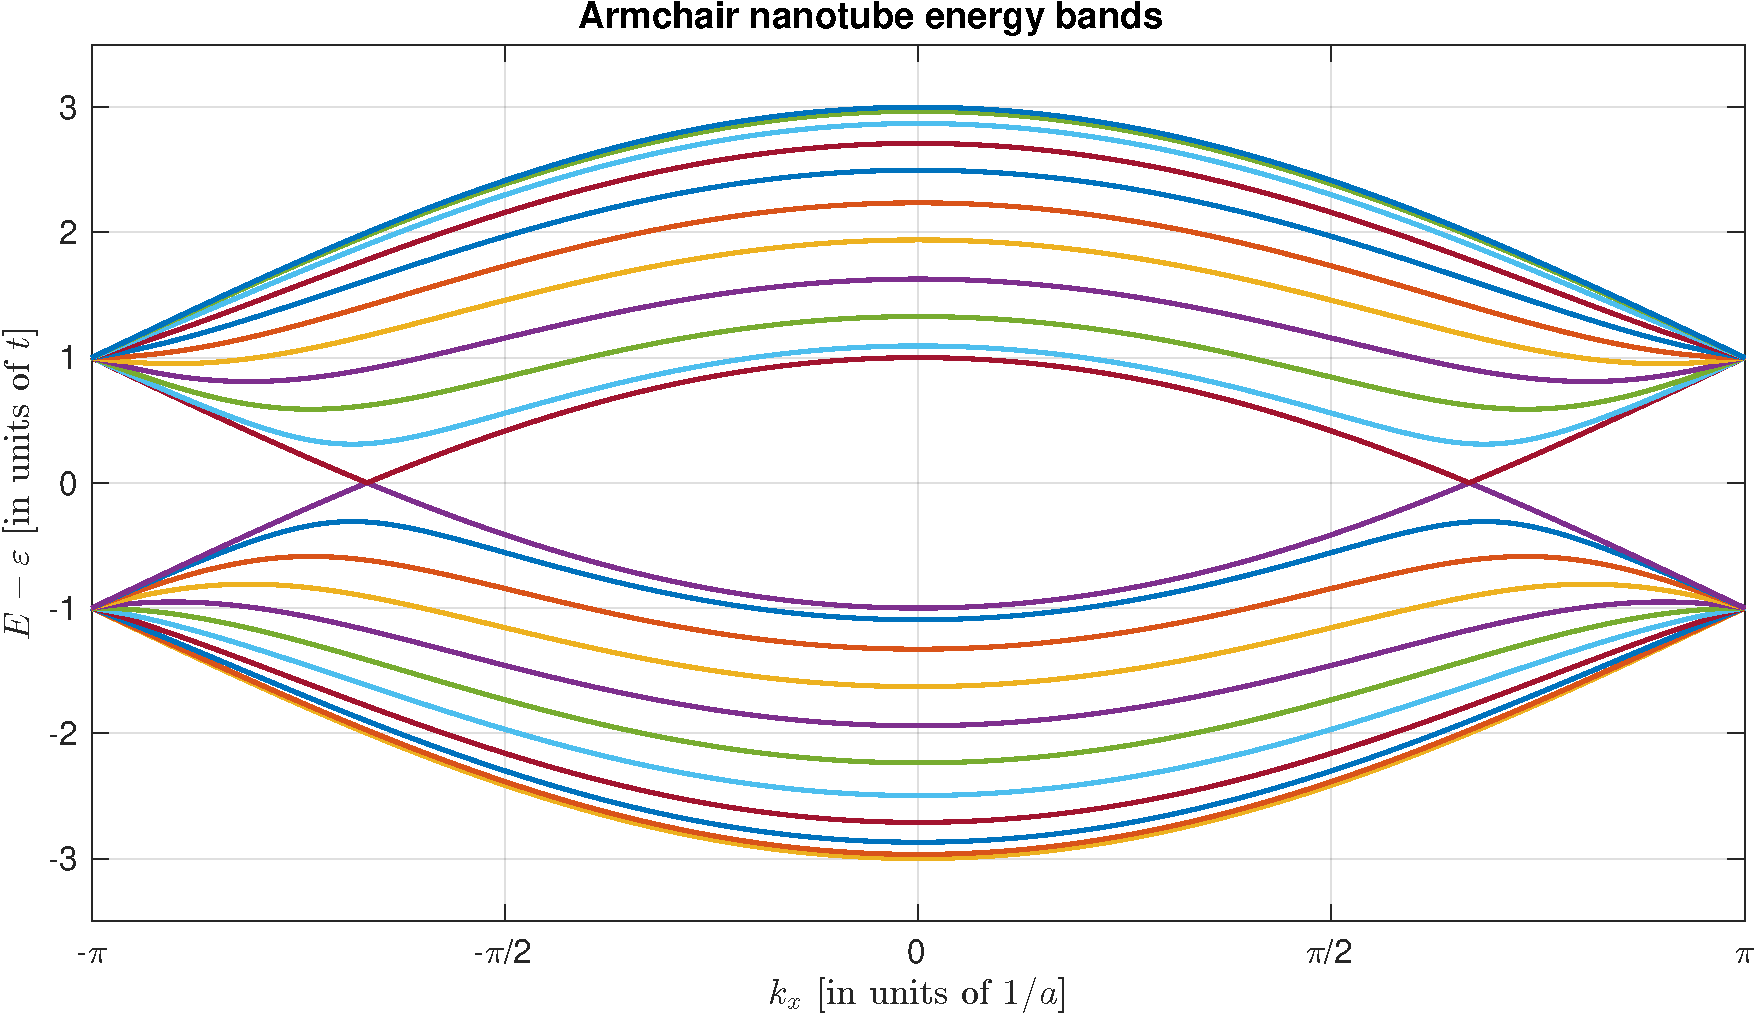
\includegraphics[width=\textwidth]{B_E_of_k}
		\caption{Plot of $E(k_x)$ for different (discrete) values of $k_y$. The values used are $N=10$, $t=1$ and $a=1$.}
		\label{fig:B_E_of_k}
	\end{figure}


\end{proof}


\end{document}